%!TEX root = ../Thesis.tex

\section*{Anhang}
\addcontentsline{toc}{section}{Anhang}
\fancyhead[R]{Anhang}

\anhangsverzeichnis

%\anhang{Quellcode}

%\subanhang{Kombinationen zwischen den Betriebsmodi}
%\label{anhang1}
%\begin{lstlisting}[caption={Code zum herstellen vordefinierter Kombinationen zwischen den Befehl Buttons}, label=Operation]
%// Logik fuer die Operation Modes in FlowChief
%//Trigger fuer die Interaktionsfenster Buttons in FlowChief
%R_TRIG_AUTO(*@\textcolor{blue}{(}@*)CLK := INOUT_LSR_FlowChief_OPCUA.Commands._AUTO(*@\textcolor{blue}{)}@*);
%R_TRIG_HAND(*@\textcolor{blue}{(}@*)CLK := INOUT_LSR_FlowChief_OPCUA.Commands._HAND(*@\textcolor{blue}{)}@*);
%R_TRIG_EIN(*@\textcolor{blue}{(}@*)CLK := INOUT_LSR_FlowChief_OPCUA.Commands._EIN(*@\textcolor{blue}{)}@*);
%R_TRIG_AUS(*@\textcolor{blue}{(}@*)CLK := INOUT_LSR_FlowChief_OPCUA.Commands._AUS(*@\textcolor{blue}{)}@*);
	
%//Sicherstellen entweder Automatik Modus oder Hand Modus aktiv
%IF R_TRIG_AUTO.Q THEN
%	// Zustaende im Automatik Modus
%	INOUT_LSR_FlowChief_OPCUA.Commands._AUTO := TRUE;
%	INOUT_LSR_FlowChief_OPCUA.Commands._HAND := FALSE;
%	INOUT_LSR_FlowChief_OPCUA.Commands._EIN := FALSE;
%	INOUT_LSR_FlowChief_OPCUA.Commands._AUS := FALSE;
	
%ELSIF R_TRIG_HAND.Q THEN
%	// Zustaende im Hand Modus
%	INOUT_LSR_FlowChief_OPCUA.Commands._AUTO := FALSE;
%	INOUT_LSR_FlowChief_OPCUA.Commands._HAND := TRUE;
%	INOUT_LSR_FlowChief_OPCUA.Commands._EIN := FALSE;
%	INOUT_LSR_FlowChief_OPCUA.Commands._AUS := TRUE;
%END_IF
	
%IF INOUT_LSR_FlowChief_OPCUA.Commands._HAND THEN
%	// Verhindern Ein und Aus Befehl gleichzeitig aktiv 
%	IF R_TRIG_EIN.Q THEN
%		INOUT_LSR_FlowChief_OPCUA.Commands._EIN := TRUE;
%		INOUT_LSR_FlowChief_OPCUA.Commands._AUS := FALSE;
%	ELSIF R_TRIG_AUS.Q THEN
%		INOUT_LSR_FlowChief_OPCUA.Commands._EIN := FALSE;
%		INOUT_LSR_FlowChief_OPCUA.Commands._AUS := TRUE;
%	END_IF
	
%ELSIF INOUT_LSR_FlowChief_OPCUA.Commands._AUTO THEN
%	// Verhindern, dass im Auto Modus Ein und Aus Befehle gesetzt werden
%	INOUT_LSR_FlowChief_OPCUA.Commands._EIN := FALSE;
%	INOUT_LSR_FlowChief_OPCUA.Commands._AUS := FALSE;
	
%ELSE
%	// Sollte kein Modus Aktiviert worden sein stelle Standard Zustand her
%	INOUT_LSR_FlowChief_OPCUA.Commands._AUTO := FALSE;
%	INOUT_LSR_FlowChief_OPCUA.Commands._HAND := TRUE;
%	INOUT_LSR_FlowChief_OPCUA.Commands._EIN := FALSE;
%	INOUT_LSR_FlowChief_OPCUA.Commands._AUS := TRUE;
%END_IF
	
%\end{lstlisting}

%\subanhang{Parametrierung}
%\label{anhang2}

%\begin{lstlisting}[caption={Parametrierung des Symbols im Funktionsbaustein}]
%// Parametrierung des Symbols
	
%// 1: Buttons ausblenden wenn fernsteuerung nicht aktiv ist
%IF NOT IN_LX_Priority THEN
%	INOUT_OPC_UA_FlowChief.Parameterization.iBlock_Commands := INT#1;
	
%// 2: Freischalten der Button und Automatik Button gruen
%ELSIF IN_LX_Priority AND FlowChief_OperationMode.FlowChief_AutoMode THEN
%	INOUT_OPC_UA_FlowChief.Parameterization.iBlock_Commands := INT#2;
	
%// 3: Freischalten der Button und Hand Button gruen
%ELSIF IN_LX_Priority AND FlowChief_OperationMode.FlowChief_HandMode THEN
%	INOUT_OPC_UA_FlowChief.Parameterization.iBlock_Commands := INT#3;
	
%	IF FlowChief_OperationMode.FlowChief_Hand_Aus THEN
%		// 4: Freischalten der Button und AUS Button gruen
%		INOUT_OPC_UA_FlowChief.Parameterization.iBlock_Commands := INT#4;
	
%	ELSIF FlowChief_OperationMode.FlowChief_Hand_Ein THEN
%		// 5: Freischalten der Button und EIN Button gruen
%		INOUT_OPC_UA_FlowChief.Parameterization.iBlock_Commands := INT#5;
%	END_IF
	
%// 0: Keine Buttons Blocken wenn Fernsteuerung aktiv ist
%ELSE 
%	INOUT_OPC_UA_FlowChief.Parameterization.iBlock_Commands := INT#0;
%END_IF
%\end{lstlisting}




%\subanhang{Herstellung des Standardzustandes}
%\label{Anhang5}
%\begin{lstlisting}[caption={Standardzustand herstellen}, label=Standard]
%//Standardzustand beim Umschalten der Prioritaet herstellen
	
%//Trigger loest einmal aus, sobald von der Lokal- zur Fernsteuerung gewecheslt wird (IN_LX_Priority wechselt von FALSE zu TRUE)
%R_TRIG_FERN(CLK:= IN_LX_Priority);
	
%//Sobald Trigger ausloest, wird der Standardzustand hergestellt
%IF R_TRIG_FERN.Q THEN
%	INOUT_LSR_FlowChiefState.Commands._AUTO := FALSE;
%	INOUT_LSR_FlowChiefState.Commands._HAND := TRUE;
%	INOUT_LSR_FlowChiefState.Commands._EIN  := FALSE;
%	INOUT_LSR_FlowChiefState.Commands._AUS  := TRUE;
%END_IF
%\end{lstlisting}


\anhang{Alte Schaltlogik}
\label{alt}
\begin{figure}[h!]
	\centering
	\begin{minipage}[t]{1\textwidth} % Breite, z.B. 1\textwidth		
		\caption{Aktuelle Schaltlogik des Funktionsbausteins} % Überschrift
		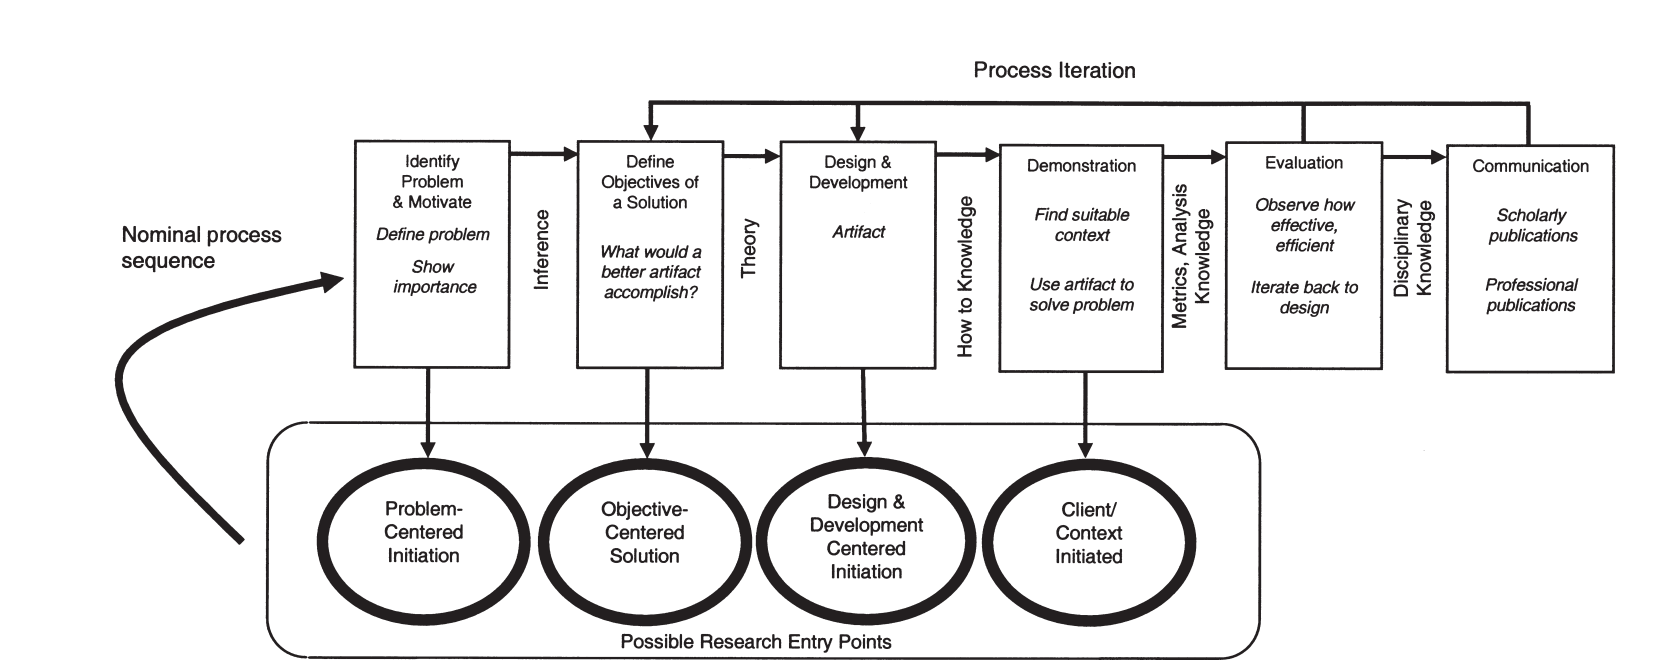
\includegraphics[width=1\textwidth]{img/dsr.png}\\ % Pfad
		\label{fig: Alter Ablauf}
	\end{minipage}
\end{figure}
\anhang{Testergebnisse}
\subanhang{Variablen nach einlesen der XML-Datei}
\label{anhang3}

\begin{figure}[hbt]
	\centering
	\begin{minipage}[t]{1\textwidth} % Breite, z.B. 1\textwidth		
		\caption{Ansicht im Anlagen Ordner} % Überschrift
		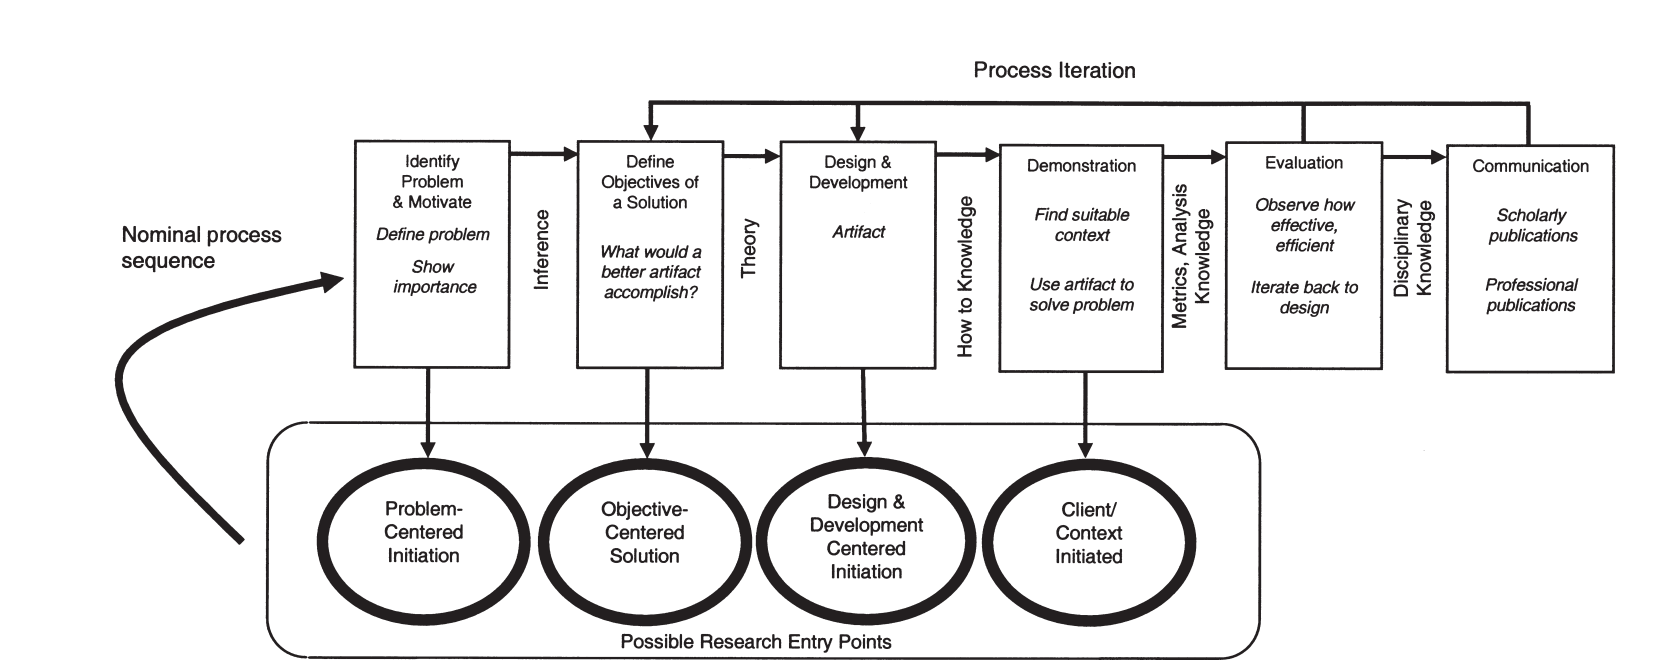
\includegraphics[width=1\textwidth]{img/dsr.png}\\ % Pfad
		
	\end{minipage}
\end{figure}

\subanhang{Ergebnisse des Zeitvergleiches}
\label{Zeitvergleich}

\begin{figure}[hbt]
	\centering
	\begin{minipage}[t]{.7\textwidth} % Breite, z.B. 1\textwidth		
		\caption{Ergebnisse des Zeitvergleiches} % Überschrift
		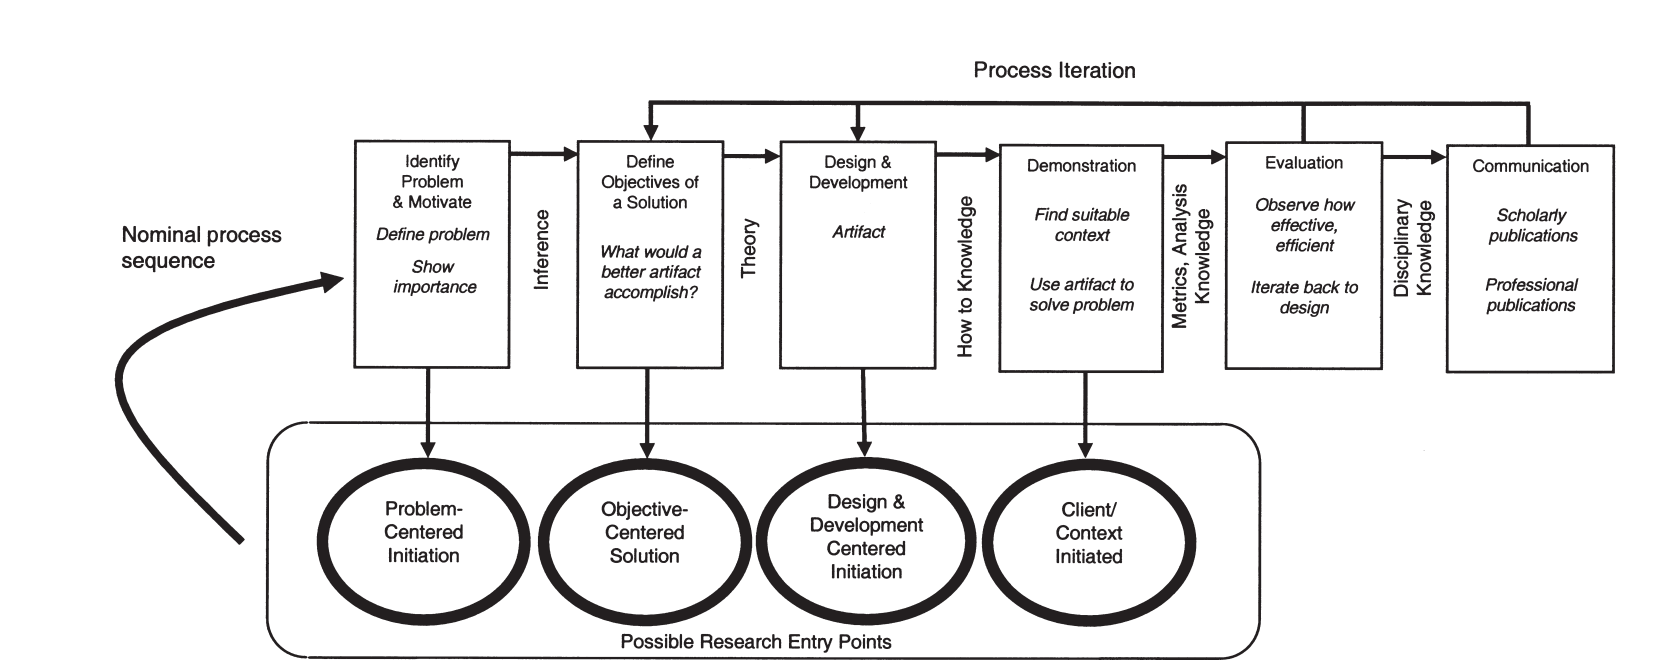
\includegraphics[width=1\textwidth]{img/dsr.png}\\ % Pfad
		
	\end{minipage}
\end{figure}
